\chapter{Programmer Documentation}

The implementation of our autonomous racing agent relies on a complex set of libraries and tools. In this chapter, we will describe the libraries and tools we used and we will briefly explain how some of them work. We will also explain how we implemented the behavior of the autonomous racing agent in the context of this setup. The installation instructions and instructions on how to deploy and use the software used and developed in this thesis are covered in the following chapter \ref{chapter:user_documentation}

\section{Robot Operating System}

Robot Operating System (ROS) is an open-source set of libraries and tools built on top of Linux. Processes running under this operating system are referred to as nodes and they can be distributed across multiple computers connected over a wired or wireless network or through a serial port. Nodes can be programmed in many different programming languages but the most common and officially supported languages are Python and C++.

Nodes communicate between each other using a publisher/subscriber pattern. A node can advertise any number of topics through which it publishes its outputs in a form of messages. It can also subscribe to topics advertised by other nodes and it can work with the received messages as its outputs. This way it is possible to create a complex system by combining many small and simple specialized nodes.

Each topic has an assigned message type which defines the structure of the data. There is a large number of standard messages which are used by authors of public libraries. This way it is often possible to replace one library with a different one without additional changes to other nodes. This can be useful for example when one sensor is replaced by a device of the same type but from a different vendor whose ROS node publishes the same standard message type. Programmers can also define their custom message types which are better suited for their application.

ROS comes with a variety of tools for debugging and visualization of the data passed through the topics. One of these tools is Rviz. It is a convenient way of visualizing the current state of the system. We use this tool to visualize the telemetry data from the vehicle on a laptop while it is driving along the racing circuit.

Further information about ROS and tutorials which describe how to work with it are available on the official website of the ROS project\footnote{https://ros.org}.
%
\section{Architecture Of The Distributed System}

The setup of our robot consists of the NVIDIA Jetson Nano board which is mounted on the vehicle, two Arduinos which are connected to the Jetson through a serial port, and a notebook which is connected to Jetson over Wi-Fi. Jetson acts as a ROS master machine, Arduinos act as an interface between Jetson and low-level hardware, and the notebook is used only to monitor telemetry data. The graph of this architecture and the connected sensors is depicted in Figure~\ref{fig:ros_diagram}.

\begin{figure}[]\centering
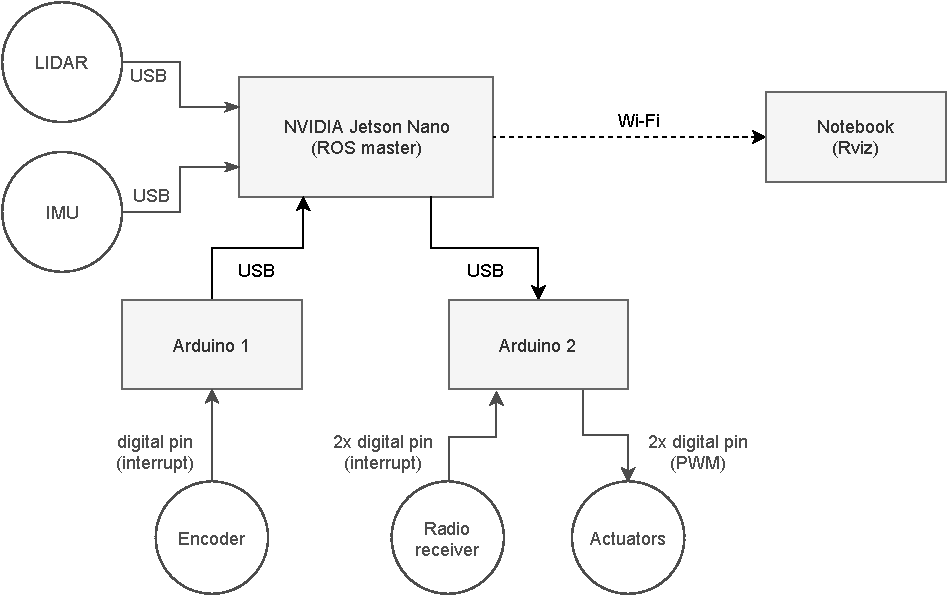
\includegraphics[width=125mm]{../img/ros_diagram.pdf}
\caption{This figure shows how the compters and sensors which make up the experimental vehicle are connected with each other and the direction of data flow between the devices.}
\label{fig:ros_diagram}
\end{figure}

The vehicle can performs two tasks: mapping and racing. In the mapping phase the vehicle creates a map of the track using the LIDAR and in the racing phase it drives autonomously around the track with the knowledge of to the map and the topology of the circuit. In the following sections we will describe how we approach these two tasks.

\subsection{Mapping}

When the vehicle is creating the map of the track, it is being controlled manually using the remote controller of the vehicle. The only sensor which is needed for this task is the LIDAR. The data from the LIDAR is being collected by a SLAM algorithm (Simultaneous Localization And Mapping) implemeted by the Hector SLAM library by a tema from the Technical University of Darmstadt.

This library performs scan matching of the LIDAR scans and it builds a 2D occupancy grid of the environment over time. For an already built part of the map and a LIDAR scan consisting of $n$ points, the task of the scan matching algorithm is to find a rigid transformation $\xi =\( p_x, p_y, \phi\)$, which gives best alignment with the already built map. The authors formulate this problem as an optimization problem for solving in \cite{HectorSlam}:

$$
\xi^* = \underset{\xi}{\arg\min}\sum_{i=1}^n\[ 1 - M\( S_i\( \xi\)\)\]^2,
$$

where $S_i\( \xi\)$ are the world coordinates of scan point $s_i$ after applying the transform $\xi$ and the function $M$ gives the value of the occupancy grid at the given coordinates.

The producer of the YDLIDAR X4 we use provides a ROS node as part of the SDK for the device. 

Hector SLAM provides a ROS node \verb|hector_mapping| which subscribes to a topic providing \verb|sensor_msgs/LaserScan|\footnote{http://docs.ros.org/melodic/api/sensor\_msgs/html/msg/LaserScan.html} messages and publishes its output in a topic of type \verb|nav_msgs/OccupancyGrid|\footnote{http://docs.ros.org/melodic/api/nav\_msgs/html/msg/OccupancyGrid.html}. When the mapping is complete, the final map can be saved into a file using a \verb|map_saver| node from the \verb|map_server| package\footnote{http://wiki.ros.org/map\_server\#map\_saver}.

\subsection{Racing}

The racing task is significantly more complicated than the mapping task. 